\documentclass{article}
\usepackage[utf8]{inputenc}
\usepackage{amsmath, amssymb, amsthm, enumerate}
\usepackage[usenames,dvipsnames]{color}
\usepackage{bm}
\usepackage[colorlinks=true,urlcolor=blue]{hyperref}
\usepackage{geometry}
\geometry{margin=1in}
\usepackage{float}
\usepackage{graphics}
\setlength{\marginparwidth}{2.15cm}
\usepackage{booktabs}
\usepackage{enumitem}
\usepackage{epsfig}
\usepackage{setspace}
\usepackage{parskip}
\usepackage[normalem]{ulem}
\usepackage{tikz}
\usetikzlibrary{positioning}
\usepackage{pgfplots}
\pgfplotsset{compat=1.13}
\usepackage[font=scriptsize]{subcaption}
\usepackage{float}
\usepackage[]{algorithm2e}
\usepackage{environ}
\usepackage{bbm}
\usepackage{graphicx}
\usepackage{titling}
\usepackage{url}
\usepackage{xcolor}
\usepackage{lipsum}
\usepackage{lastpage}
\usepackage[colorlinks=true,urlcolor=blue]{hyperref}
\usepackage{multicol}
\usepackage{tabularx}
\usepackage{url}
\usepackage[nottoc]{tocbibind}
\usepackage{setspace}




\begin{document}
\begin{spacing}{1}

\section*{}
\begin{center}
  \vspace{0.5em}
  \centerline{\textsc{\Large Course Project}}
  \vspace{1em}
  \textsc{\large CMU 24-623: Molecular Simulation of Materials (Fall 2017)} \\
  \vspace{1em}
  \textsc{\large Junrong Huang, Hongyi Liang} \\
\end{center}



\section*{}
\begin{center}
\centerline{\textbf{\Large Compare different thermostats for NVT MD simulations}}
\end{center}

\section*{}
\textbf{Abstract: } Molecular dynamic simulations have become a standard tool in multiple dynamic systems. In most of the practical simulations some parameters like temperature/pressure need to remain constant. People have come up with different methods called thermostats to keep the temperature constant. In our simulations, we are going to compare several well-known thermostats which are developed around 1980s and give an overall judgement about their advantages under several conditions.

\section*{}
\textbf{Keywords: } Thermostat, Molecular Dynamics Simulations


\section{Introduction}
Molecular dynamic simulations have played an increasingly important role in the field of materials science including theoretical and experimental work. Molecular dynamic simulation is a computational tool concerning about the modeling of molecular structure, the atomistic or molecular assemblies and the interactions between atoms. These simulations will be useful in studying atomic or molecular structures and properties. 

Traditionally, molecular dynamic simulations are served as a bridge between theory and experiment or complementary validations of conventional laboratory works. We can test a theory by simulations using a particular model and compare the results with experimental results using the same model or comparing two different models directly to figure out good simulation methods. It’s essential and important to choose a good model before performing simulations. Furthermore, we may carry out some simulations which are tough and even impossible in laboratory (like a system which is working under extreme temperature or pressure). But recent research show that with the development of distributed and parallel computing techniques, molecular dynamic simulations can also produce some innovative and informative views which can in turn help promote further experimental research and provide substantial benefit to computational materials science. In this sense, we can even reveal some hidden regulations based on our predictions. Currently, one of the challenges arise in molecular dynamic simulations is that molecular simulation is inherently a multi-discipline research so it requires extensive knowledge and collaboration of some problem-specified fields which are beyond the boundaries of each individual field.

Two main techniques used in molecular dynamic simulations are molecular dynamics(MD) and Monte Carlo method(MC). There are great potentials to combine the features of these two methods to form a hybrid method. In practice, Monte Carlo simulations are proposed to simulate the probability of different outputs because of the random variables by random sampling to obtain numerical results. Monte Carlo simulations is fit for the problem which can be described by probability distribution theory.

In our project, we will use Monte Carlo methods to initialize atom positions (atom numbers are constant) in successive simulation process. 


\section{Paper Summary and Objectives}
In molecular dynamic simulations, typically we will numerically solve the Newtonian motion equations for a collection of particles. In practice, it’s desirable to keep the number of particles, the volume of our systems as well as the temperature/pressure to be constant to simulate a NVT ensemble which has empirical meaning in experimental work. Also, the energy of the system is conserved.  Usually, it’s straightforward and easy to restrict a fixed number of atoms in a fixed-volume box to make N and V constant. But when it comes to temperature/pressure, there will be much more factors that we need to consider. 

Since 1980, extensive research has been conducted to figure out how to remain constant temperature for a NVT system. People proposed that the most effective and easy-understanding way is introducing thermostats into molecular simulations. 

Multiple thermostats have been device in purpose of remaining system temperatures. For example, on one hand, in (I) Hans C. Anderson’s paper~\cite{1}, first he went over some basic questions and fundamental ideas in molecular dynamic simulations like what’s the goal of molecular simulations define some sequences of configurations generated by a specific stream of algorithms. Then he proposed that when studying instances like dilute solutions which is worth studying under constant temperature/pressure with appropriate energy fluctuations, it’s better to use Monte Carlo method rather than molecular dynamics even the MD methods can give some information about time-dependence fluctuations. 

In Anderson’s work, he introduced some periodic conditions so that he can apply his molecular dynamic simulations to bulk fluid. Since a small group (50-100) of particles are subject to the surrounding energy fluctuations, even the whole system is at constant temperature, the energy of the system still fluctuates. One possible solutions to introduce energy fluctuations mechanism is by inventing one or more additional degrees of freedom (it’s also the case in keeping the constant pressure case). He imposed instantaneous stochastic forces on atoms of the sample, without introducing surface effects, so that the kinetic energy will change. These stochastic collisions which obey Poisson process can affect the momentum of a single particle, while each collision is statistically un-correlated. Each time the state of the system can evolve according to two parameters: T which is the desired temperature and $\nu$ is the mean rate at which each particle suffers collisions. Also, there are some probabilities that for a given particle to suffer a stochastic collision in some small-time interval.

In Anderson’s system, because he will perform a finite number of significant figures, so the numbers of states are countable, which means he can apply Markov chains with a countable number of states. For certain Markov chains, the probability that the simulated system is in each state at time t approaches a limit, and this limiting probability distribution is independent of the initial state of the system. 

Finally, he proved that even for the system with large enough number of particles, most of the molecules will be moving according to the conservative equations of motion for a closed system so his thermostat still works well. And the time averages of properties are equal to averages over the given ensembles with given number of particles in a volume element while taking the influence of the surroundings into account.

On the other hand, Berendsen~\cite{2} el at first evaluated the job done by other researchers like the Anderson thermostat and Hoover thermostat. They pointed out that there still exist two problems, first would be the inaccuracy in algorithm can produce drift in pressure or temperature that is not stabilized, and the reference pressure/temperature does not appear in the equations. Second would be the problem that Hamiltonian does not represent a physical system so the extent of error cannot be easily measured. In this sense, in order to obtain realistic simulations of physical systems, even though mathematically consistent equations can be obtained, using nonphysical Hamiltonian is questionable.

To solve preceding problems, Berendsen and his colleagues proposed a different approach called weak coupling to an external bath instead of modifying the Hamiltonian. Because their methods approximate the perturbation that could appear in a practical experiment, and the coupling strength can be varied, the effect of the coupling can be easily evaluated and controlled.
Therefore, they introduce a fixed reference temperature to a system coupling with a heat bath. They simply modify the equations of motion by inserting stochastic and friction term. And their models correspond to frequent collisions with light particles that form an idea gas at desired temperature physically.

$$m_i\dot v_i=F_i-m_i\gamma_iv_i+R(t)$$
$$<R_i(t)R_j(t+\tau)=2m_i\gamma_ikT_0\delta(\tau)\delta_{ij}>$$

Then the time dependence of T can be derived from the derivative of the total kinetic energy, they can reach an expression:

$$\left(\frac{dT}{dt}\right)_{bath}=2\gamma(T_0-T)$$

And the global additional temperature coupling can be accomplished with:

$$m_i\dot v_i=F_i+m_i\gamma\left(\frac{T_0}{T}-1\right)$$

Combining all the expression about and solve the deferential equations, they proposed a thermostat:

$$\lambda=1+\frac{\Delta t}{2\tau_T}\left(\frac{T_0}{T}-1\right)$$

$$\lambda=\left[1+\frac{\Delta t}{\tau_T}\left(\frac{T_0}{T}-1\right)\right]^{1/2}$$

By using their thermostat in simulations process, although short coupling time constants greatly influence fluctuations, average thermodynamic quantities are not disturbed even for short time constants.  So their method described here to couple a simulated system loosely to a constant temperature and/or pressure bath has proved to be reliable and easy to implement.

In our final project, given the fact that some effective thermostats have already been used in practice, we are not going to propose other thermostats or methods to remain constant temperature in a NVT system. Instead, we notice that there lack of some substantial research in comparing different thermostats with different models even though they have similar results. In our simulations, we will evaluate different thermostats from mathematical and algorithmic perspectives, and give a judgement about their behavior and performance under multiple conditions, and provide some insights into how to improve those thermostats. In particular, we will compare the previously mentioned thermostats with Nóse-Hoover thermostat which consists of only one imaginary particles in the heat bath. We have already implemented it in homework problems. By using a Nóse-Hoover thermostat, our practical NVT system can achieve satisfactory and statistically constant temperature conditions. In this sense, a Nóse-Hoover thermostat can be the reference and standard when judging the effects of other thermostats.



\section{Implementation}

In this course project we implemented 3 thermostats, i.e., velocity rescaling, Andersen thermostat, Berdersen thermostat to the liquid argon system. The Nóse-Hoover thermostat had already been implemented in homework and resented a thermo heat capacity simulation result as $503.069J/(kg\cdot K)$. Therefore, we implemented the other three kinds of thermostats and discuss how they perform, and can they provid a reasonable thermo values in the simulation process.

We simulated the process that the system was started at an initial temperature as 50K and ended at the thermostat temperature 100K for 200 simulation time units. The initialization of the system was set as: initial position was initialized with {\it "liquid256.txt"}; he initial velocities of each particles were generated according to Maxwell-Boltzmann velocity distributiion at initial temperature set as $50K$.

The symbols we used in this implemenation section is listed:

{\it $N$ - number of particles in the system, i.e., 256; $t$ -  step; $\delta t$ - dimensionless time step, set as 0.002 in this project; $m_i$ - the mass of particle $i$, is set as 1 in the dimensionless space for every argon atom; $v_i$ - velocity of particle $i$; $T_0$ - thermostat temperature; $T$ - kinetic temperature of the system; $K$ - kinetic energy of the system; $\lambda$ - velocity rescaling factor at step $t$; $\gamma$ - heat flow variable; $\tau$ - Time constant of the coupling to the heat bath}

\vspace{1.5em}
\textsc{\Large Velocity Rescaling}

In order to control kinetic temperature, the most direct way is to rescale the velocity at each time step since the kinetic is directly affected by the kinetci energy of a system:

$$K=\sum_i^N \frac{1}{2}m_iv_i^2, T=\frac{2K}{3(N-1)k_B}$$

The idea of velocity rescaling:

$$v_i^{new}=\lambda v_i^{old}, \lambda=\sqrt{\frac{T_0}{T}}$$

This procedure leads to rapid energy transfer between different degrees of freedom of the particle. Resetting of velocities may be required from time to time, which means, we have to do the rescaling after each verlet loop to keep the system stabled at the thermostat set temperature. The detailed algorithm is shown below:

$$\begin{aligned} 
& 1. v_{i}(t+\Delta t/2)=v_{i}(t)+F_{i}(t)\Delta t/(2m_i) \\ 
& 2. r_{i}(t+\Delta t)=r_{i}(t)+v_{i}(t+\Delta t/2)\Delta t \\ 
& 3. v_{i}(t+\Delta t)=v_{i}(t+\Delta t/2)+F_{i}(t+\Delta t)\Delta t/(2m_i) \\
& 4. \lambda(t)=\sqrt{T_0/T(t)} \\
& 5. v_{i}(t+\Delta t)=\lambda(t) \times v_{i}(t+\Delta t)
\end{aligned}$$

\vspace{1.5em}
\textsc{\Large Andersen Thermostat}

The Andersen approach couples velocity of a particle to a heat bath via stochastic collisions. Generate canonical ensemble: less realistic dynamics and thus not used for computing dynamic quantities (e.g. diffusion coefficients, lifetime of water hydrogen bonds)

Procedure of Andersen algorithm:

starting from intial conditions integrate the equations of motion for $\delta t$

particles that undergo collisions with the heat bath are selected
the probability of selecting a praticle during the integration time step $\delta t$ is $v\delta t$, where v is the probability of collision

new velocites for selected particles are chosen at random from Maxwell- Boltzmann distribution at the desired temperature; all other particles remain unaffected.

Detailed algorithm:


$$\begin{aligned} 
& 1. v_{i}(t+\Delta t/2)=v_{i}(t)+F_{i}(t)\Delta t/(2m_i) \\ 
& 2. r_{i}(t+\Delta t)=r_{i}(t)+v_{i}(t+\Delta t/2)\Delta t \\ 
& 3. v_{i}(t+\Delta t)=v_{i}(t+\Delta t/2)+F_{i}(t+\Delta t)\Delta t/(2m_i) \\
& 4. if\ rand<(\tau \Delta t):v_{i}(t+\Delta t)=randGaussian(0, v_{T_{set}}, \sigma)\\ 
\end{aligned}$$


\vspace{1.5em}
\textsc{\Large Berendsen Thermostat}

To maintain the temperature the system is coupled weakly to an external heat bath with a fixed temperature($T_0$)

Detailed algorithm:

$$\begin{aligned} 
& 1. v_{i}(t+\Delta t/2)=v_{i}(t)+F_{i}(t)\Delta t/(2m_i)+\gamma(T_0/T-1)v_i(t)\Delta t/2 \\ 
& 2. r_{i}(t+\Delta t)=r_{i}(t)+v_{i}(t+\Delta t/2)\Delta t \\ 
& 3. v_{i}(t+\Delta t)=v_{i}(t+\Delta t/2)+F_{i}(t+\Delta t)\Delta t/(2m_i)+\gamma(T_0/T-1)v_i(t+\Delta t/2)\Delta t/2 \\
& 4. \lambda(t)=\sqrt{1+\delta t/\tau(T_0/T(t)-1)}\\ 
& 5. v_i^{new}=\lambda v_i^{old}
\end{aligned}$$

 
when $\tau \to \infty$ - Berendsen thermostat does not work (sampling microcanonical ensemble)

when $\tau = \delta t$ - Berendsen thermostat turns into a simple scaling scheme

when $\tau$ is very small the coupling to the heat bath is large and there is a significant energy exchange between the system and the thermal bath efficient does not lead to the canonical distribution


\vspace{1.5em}
\textsc{\Large Nóse-Hoover Thermostat}

Nóse-Hoover:

Nóse-Hoover proposed that the bath is an integral part of the system by adding a fictitious degree of freedom to the physical system. As a result the system does possess $6N+1$ degrees of freedom in $\tau$ space.

$$\dot r_i(t)=\dot v_i(t)$$
$$m_i\dot v_i(t)=F_i(t)-\zeta(t)m_i\dot v_i(t)$$

The heat flow variable $\zeta$ has its own equation of motion enabling fluctuations of temperature:

$$m_t\dot \zeta_t(t)=2v^Tmv-gk_BT_0$$

$m_t$ - fictitious mass; $g$ - number of degrees of freedom in the system

In this way, the system Hamiltonian is conserved:

$$H(r_i, p_i, \zeta)=K(p_i)+U(r_i)+\frac{1}{2}(m_t\zeta_t^2)+\frac{3}{2}Nk_BT_0x_t$$

The Nóse-Hoover thermostat allows the temperature to fluctuate about the average value and controls the oscillations of temperature, and it can lead to canonical distribution.

The algorithm is practiced in homework and the heat capacity calculation result is reasonable. We will use this value($503.069J/(kg\cdot K)$) to compare with the simulation result of heat capacity from the other three thermostats.


\section{Results}

We run the 3 thermostats on the system and tested the heat capacity of the system.

$$<T>=\left[\frac {<(E-<E>)^2>}{3(N-1)k_Bc_v}\right]^{1/2}$$

$$C=\frac {3c_v}{m}=\frac {<(E-<E>)^2>\cdot \epsilon ^2}{m(N-1)k_B<T>^2}$$

where $<T>=100K$, $<E>=\bar E$, $m=6.63\times 10^{-26}kg$, $\epsilon = 1.67\times 10^{-21} J$ for argon.

We used time-averaged temperature and time-averaged energy to represent the ensemble-averaged descriptors.

\vspace{1.5em}
\textsc{\Large Velocity Rescaling}

The energy oscillations and temperature oscillations w.r.t time step is shown below:

\begin{figure}[htbp]
  \centering
  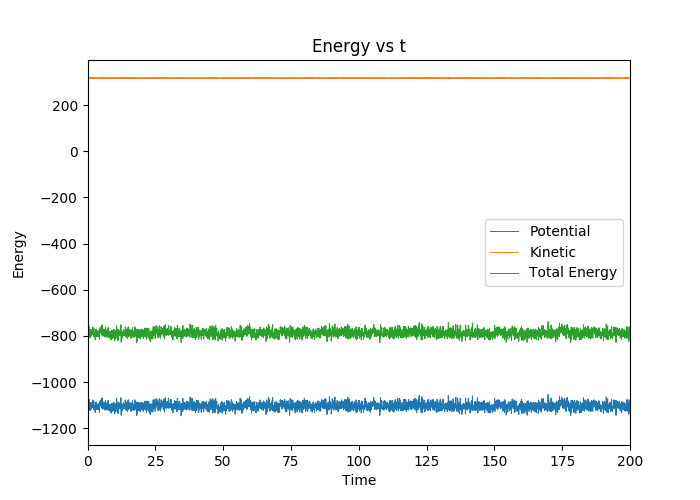
\includegraphics[width=0.45\textwidth]{vs/test/Energy.png}
  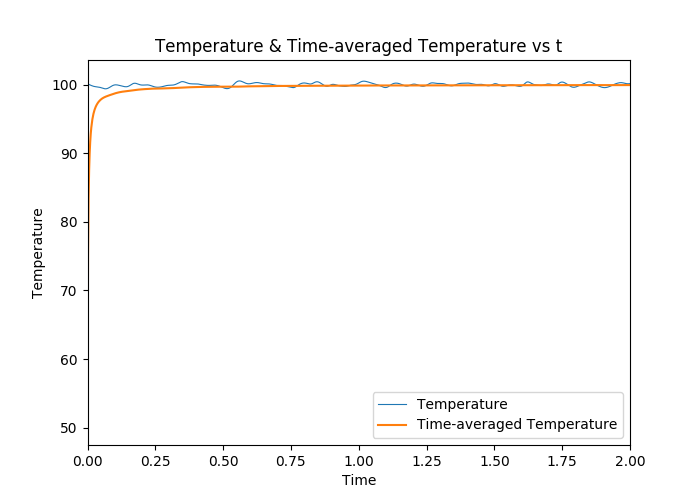
\includegraphics[width=0.45\textwidth]{vs/test/T&aT_s.png}
\end{figure}

We can see that the kinetic energy is locked as a constant since we applied the velocity rescaling algorithm after each verlet loop.

Then we calculated the heat capacity with the oscillations of energy:

$$<E> = -787.69936 (dimensionless)$$
$$C_v = 197.246J/(kg\cdot K)$$

The thermovalue calculated by this simulation is much smaller than the real value

In addition, we also checked that the system's momenta is conserved:

\begin{figure}[htbp]
  \centering
  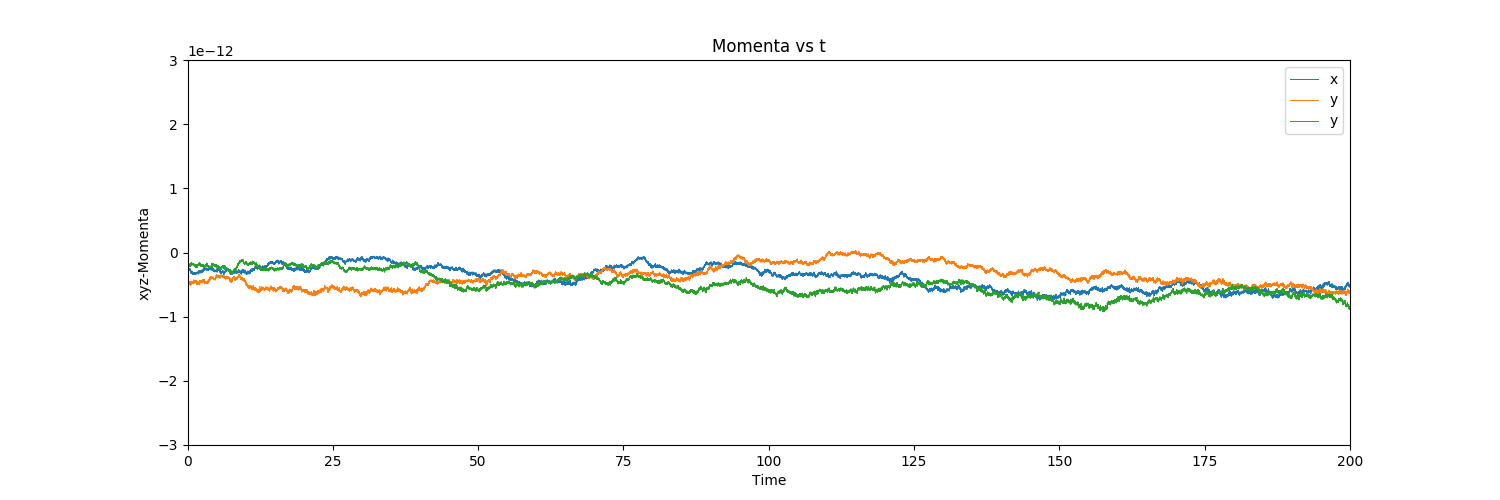
\includegraphics[width=1\textwidth]{vs/test/Momenta.png}
\end{figure}


\vspace{1.5em}
\textsc{\Large Andersen Thermostat}

In Andersen thermostat, the parameter $\nu$, the collision frequency, or or collision time $tau=1/nu$ can be tuned to adjust the coupling degree of the system with the thermostat. The relationship between $\nu$ and the behavior of a system is shown below, larger $\nu$ will lead to a greater coupling between the system and the thermostat, i.e. the system will reach its equilibrium in a shorter period.

\begin{figure}[htbp]
  \centering
  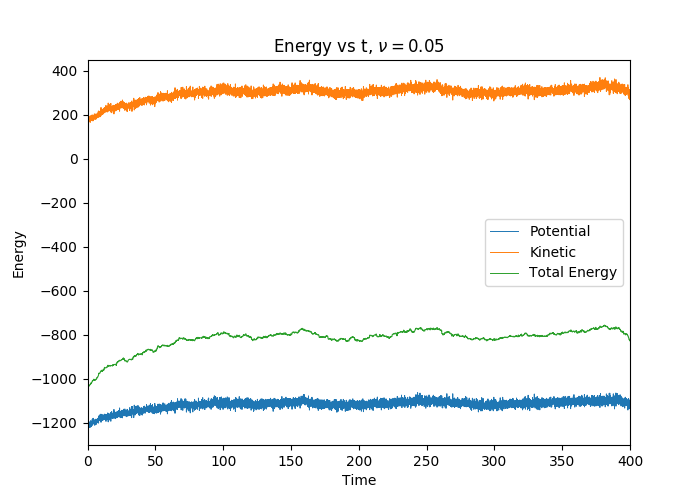
\includegraphics[width=0.3\textwidth]{andersen/nu005/test/Energy.png}
  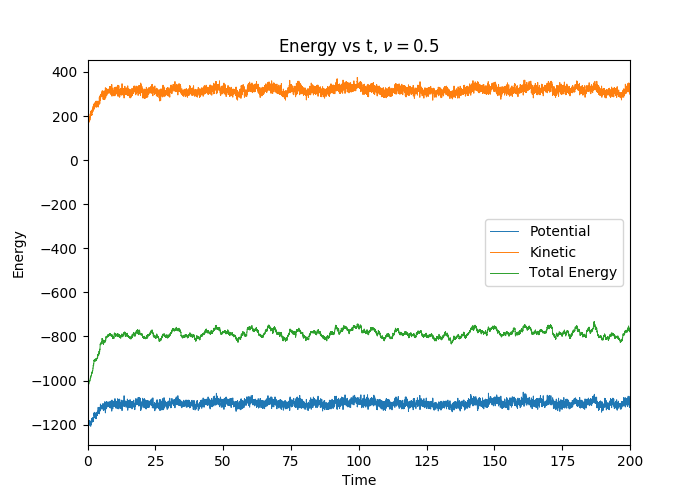
\includegraphics[width=0.3\textwidth]{andersen/nu05/test/Energy.png}
  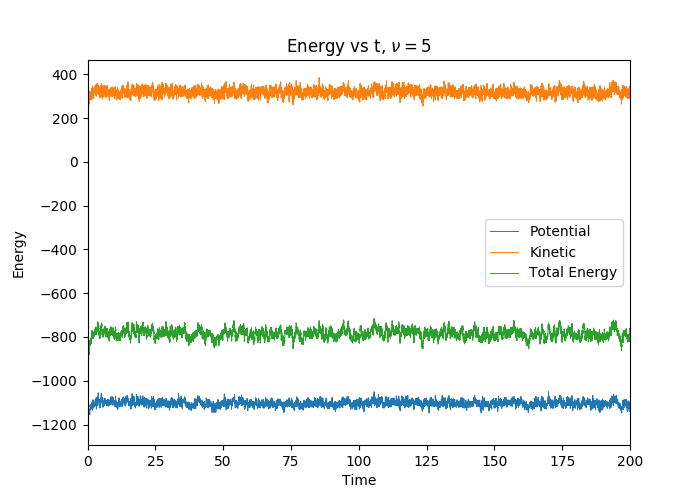
\includegraphics[width=0.3\textwidth]{andersen/nu5/test/Energy.png}
\end{figure}

\begin{figure}[htbp]
  \centering
  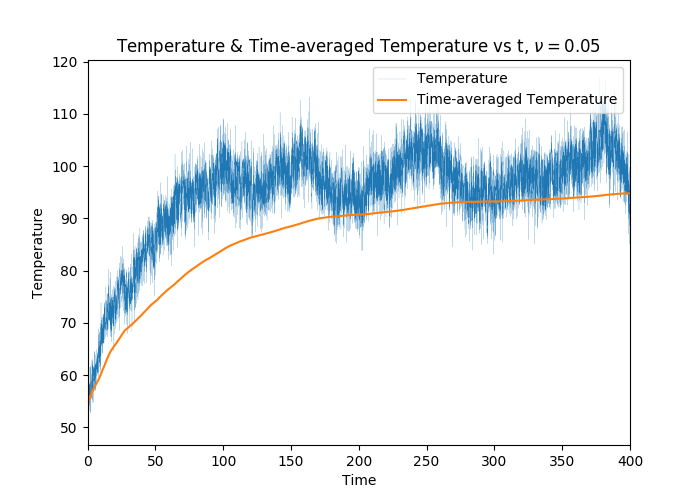
\includegraphics[width=0.3\textwidth]{andersen/nu005/test/T&aT.png}
  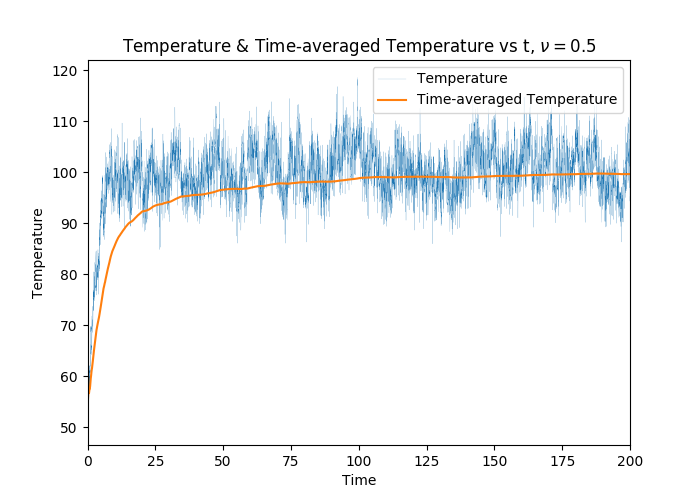
\includegraphics[width=0.3\textwidth]{andersen/nu05/test/T&aT.png}
  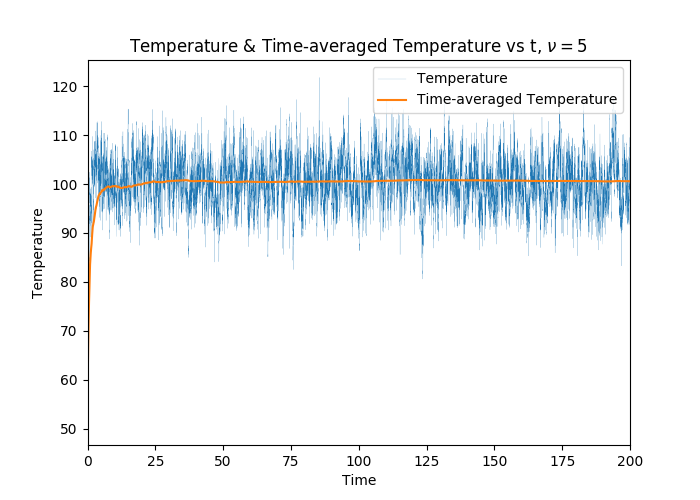
\includegraphics[width=0.3\textwidth]{andersen/nu5/test/T&aT.png}
\end{figure}

We calculated the heat capacity of each $\nu$ for the Andersen thermostat.


\begin{center}
Heat capacity with different $\nu$

\begin{tabular}{lccc}
\hline
$\nu$ & 0.05 & 0.5 & 5\\ \hline  
$<E>$(dimensionless) & -806.910350319 & -786.548732441 & -784.699660184 \\
$C_v(J/(kg\cdot K))$ & 854.373671061 & 319.110878322 & 464.649088522 \\\hline
\end{tabular}
\end{center}

As the $\nu$ values become larger, the heat capacity grows larger and more accurate to the realistic value. The value of $\nu=0.05$ is extreamly large because of the system has not reached its equilibrium even if we set the simulation time twice as the others. However, the Andersen thermostat's result of heat capacity is more closer to the real data from experiments than the velocity rescaling.

Meanwhile, the momenta is not conserved since we re-distributed the velocity with the Maxwell-Boltzmann velocity distribution. We plotted the histograom of the momenta, and the simulation results obey the Boltzmann distribution.

\begin{figure}[htbp]
  \centering
  \includegraphics[width=0.3\textwidth]{andersen/nu005/test/momenta.png}
  \includegraphics[width=0.3\textwidth]{andersen/nu05/test/momenta.png}
  \includegraphics[width=0.3\textwidth]{andersen/nu5/test/momenta.png}
\end{figure}


\vspace{1.5em}
\textsc{\Large Berdersen Thermostat}

In Berdersen thermostat, we tunned the parameter $\tau$ as the coupling factor to see the system performance with applied to a thermostat.


\begin{figure}[htbp]
  \centering
  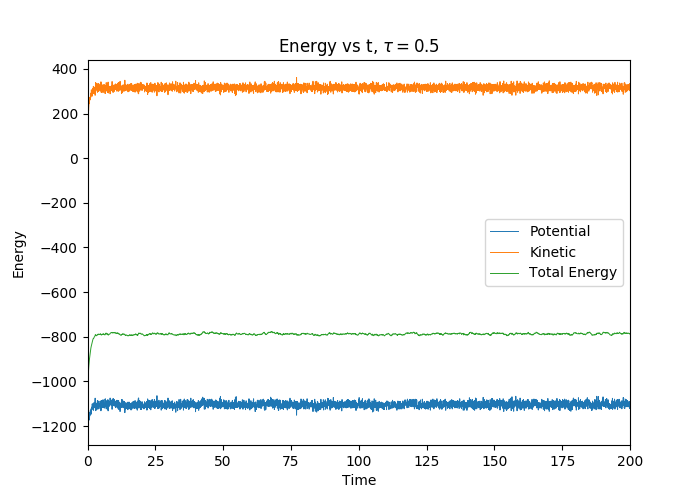
\includegraphics[width=0.3\textwidth]{berendsen/tau05/test/Energy.png}
  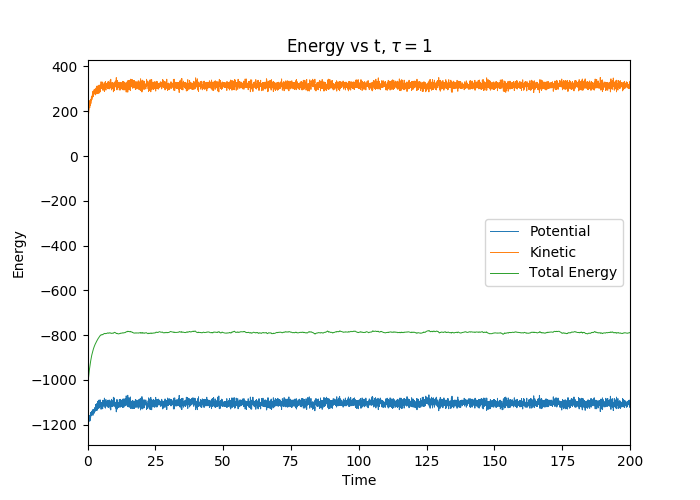
\includegraphics[width=0.3\textwidth]{berendsen/tau1/test/Energy.png}
  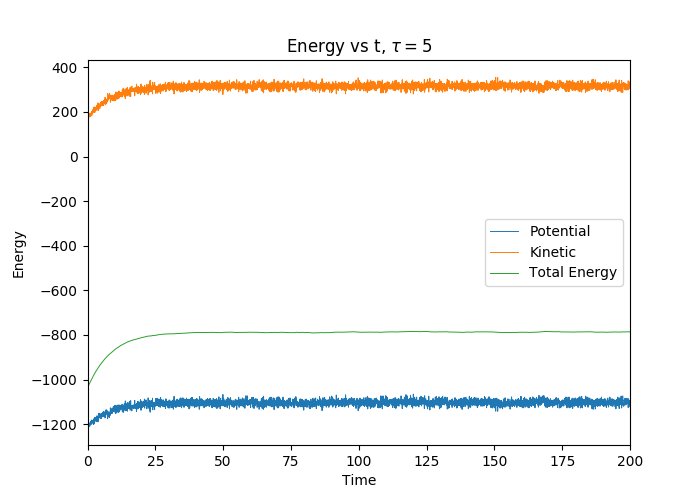
\includegraphics[width=0.3\textwidth]{berendsen/tau5/test/Energy.png}
\end{figure}

\begin{figure}[htbp]
  \centering
  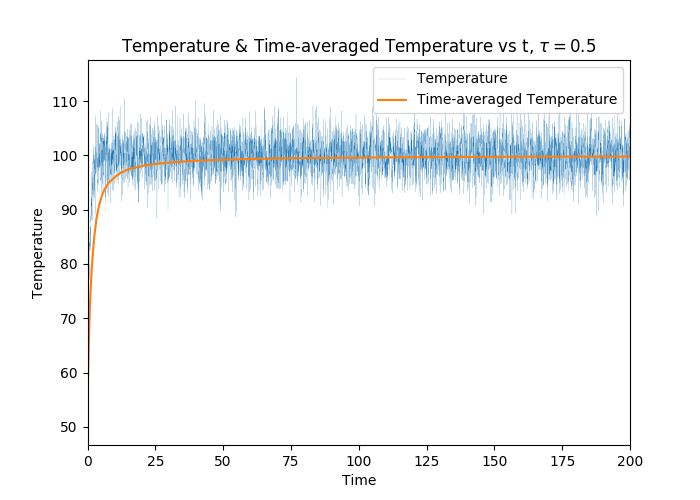
\includegraphics[width=0.3\textwidth]{berendsen/tau05/test/T&aT.png}
  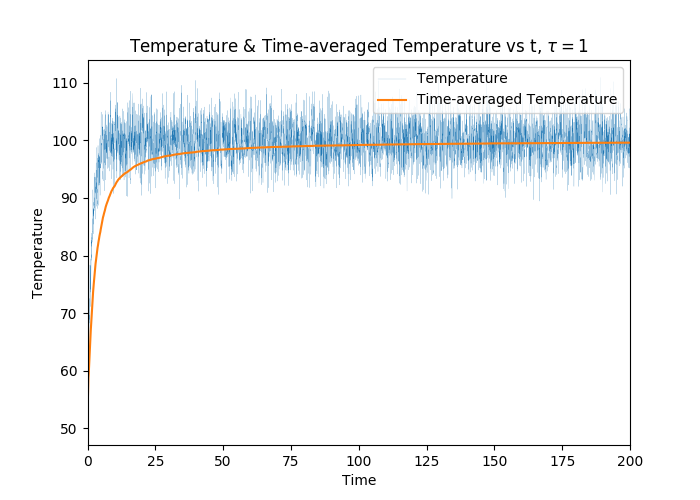
\includegraphics[width=0.3\textwidth]{berendsen/tau1/test/T&aT.png}
  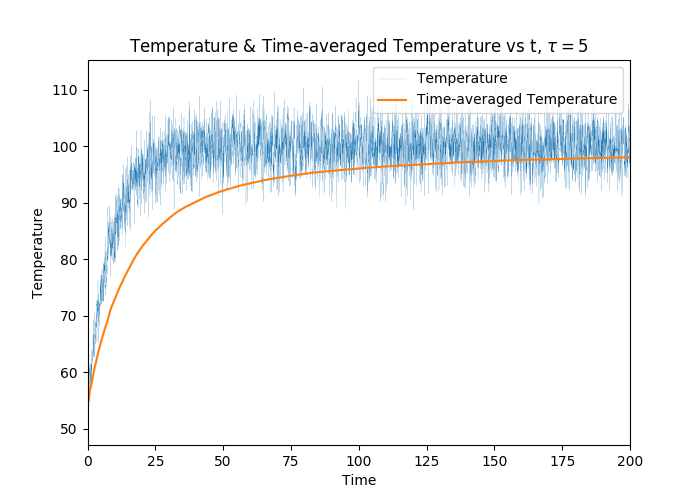
\includegraphics[width=0.3\textwidth]{berendsen/tau5/test/T&aT.png}
\end{figure}

As the $\tau$ becomes larger, the system approaches its equilibrium slower. We calculate the thermo heat capacity with different given $\tau$:


\begin{center}
Heat capacity with different $\tau$

\begin{tabular}{lccc}
\hline
$\tau$ & 0.5 & 1 & 5\\ \hline  
$<E>$(dimensionless) & -787.466874779 & -787.838028221 & -791.047653768 \\
$C_v(J/(kg\cdot K))$ & 14.1416209612 & 7.83970912134 & 152.708707285 \\\hline
\end{tabular}
\end{center}

As shown in the table above, the heat capacity is too small comparing to the real data. It is because that the Berdersen thermostat is still a velocity rescaling method with a couping factor that describes how fast the system react to the thermostat. It cannot correctly reflect the real heat transfer.


\end{spacing}
\begin{thebibliography}{1}

\bibitem{1} 
\href {http://aip.scitation.org/doi/10.1063/1.439486}{Molecular dynamics simulations at constant pressure and/or temperature Andersen, H. C. (1980). The Journal of Chemical Physics. 72 (4): 2384.}

\bibitem{2} 
\href {https://doi.org/10.1063/1.448118}{Molecular dynamics with coupling to an external bath H. J. C. Berendsen, J. P. M. Postma, W. F. van Gunsteren, A. DiNola, and J. R. Haak}

\bibitem{3}
\href {http://www.sciencedirect.com/science/article/pii/0375960195009736?via%3Dihub}{Kinetic moments method for the canonical ensemble distribution
William G.Hoover. Brad LeeHolian.}

\bibitem{4}
\href {https://doi.org/10.1007/b99427}{Thermostat Algorithms for Molecular Dynamics. Simulations, Laboratorium für Physikalische Chemie, ETH Zürich, CH-8093 Zürich, Switzerland}

\bibitem{5}
\href {http://www.math.ucsd.edu/~y1zhao/ResearchNotes/ResearchNote007Thermostat.pdf}{Brief introduction to the thermostats, Yanxiang zhao, UCSD}

 
\end{thebibliography}
\end{document}
